% Define table for personas.
\newcommand{\persona}[4]{%
    \textbf{#1}
    \small\begin{tabular}[t]{|p{.8in} | p{1.5in}|}
        \hline
        \textbf{Preferences} & #2 \\\hline
        \textbf{Pain Points} & #3 \\\hline
        \textbf{Goals} & #4 \\
        \hline
    \end{tabular}
    \vspace{4pt}
}


\chapter{Introduction}
\label{chap:introduction}

\section{Background}
\label{section:background}

In universities and campuses, cafeteria food is a staple for students' lifestyles.
It is important that a university cafeteria has various cuisines and food choices to choose from in order to accommodate
any diet a student prefers. However, the abundance of options paves way for students to spend their valuable time in choosing
their meal within their budget and time constraints. The result of students choosing can lead to mixed responses;
while some feel satisfied with their meal choices, others feel regretful for their order.
Causes such as taste, value and personal bias can be the reasons for dissatisfaction in cafeteria food. \cite{marquisetal:2018}

During Kasetsart University's lunch hours,
most of the cafeteria will be full of students and taking too long to choose their meal is not a viable option
since some students have only an hour of lunch time before their studies. The motivation of this project is to simplify
the decision-making process for students in choosing meals from various food stalls within
the cafeterias at Kasetsart University so they can save time and enjoy their meal.

% Consider switching paragraph 2 and 3.

Students get guidance on what they should get for their meals by asking their friends or other students on campus.
This kind of conversation can happen anywhere---in the cafeteria, in a classroom, on the campus grounds or on an online messaging application etc.
However, this is not always reliable for each students' own preferences, as each individual can have different perspectives
and experiences on meal choices. Additionally, Kasetsart University does not have a publicized, centralized data source
for food stalls in cafeterias. As a result, no food guide application tailored to Kasetsart University's students
has been made due to lack of information on the aforementioned food stalls.

\section{Problem Statement}
\label{section:problem-statement}

The problem statement for KU Eater addresses the challenge that Kasetsart University students face
when it comes to daily meal selection. With a myriad of dining options on campus, students often struggle to make choices
that align with their dietary preferences, nutritional needs, and time constraints. The complexity of this decision-making
process can lead to meal dissatisfaction and a negative impact on their academic performance and overall campus experience.
Moreover, there are currently no solution that is tailored to simplification and personalization of
KU students' processes of choosing meals.

\section{Solution Overview}
\label{section:solution-overview}

KU Eater proposes a solution by being a web-based food guide application that is usable on any platform that is connected to the internet and,
is tailored to Kasetsart University students with four prominent features and additional features to solve the problem,

\subsection{Prominent Features}
\label{subsection:main-features}

\begin{enumerate}[leftmargin=80pt]
    \item \textbf{Personalized food recommendation:} A system with pre-trained machine learning model to predict
    dietary preferences based on past attendances to Kasetsart University's cafeterias. As well as,
    showing trending meal choices by the other students using this application.
    \item \textbf{Keyword-based search for menus:} A machine learning-based search system that can classify keywords
    in the search term to find accurate food stalls that can serve meals according to user input.
    \item \textbf{Food stall reviews and rating:} A system that allows students to open discussions on their opinions
    of food stalls and the food choices they have. With written reviews, students can gain more context.
    The reviews also help with their consideration of ordering a meal.
    \item \textbf{Personal dietary behavior analysis:} KU Eater keeps track of cafeteria use patterns and reviews
    written by each user to help refine personal recommendations.
\end{enumerate}

\subsection{Data Acquisition}
\label{subsection:data-acquisition}

\begin{enumerate}[leftmargin=80pt]
    \item \textbf{Data acquisition for food stalls in Kasetsart University} \\%
        Due to lack of existing data of food stalls in cafeterias on KU, an employment of data acquisition method is required.
        \begin{enumerate}
            \item Interviewing with information holder---interviews and surveys with stall owners is our
            primary source of data, as it is the most accurate method to acquire data.
            \item Optical character recognition on menu items---all stalls have menu of food items at in front of the stall.
            We can use an character recognition technique to extract information such as, menu item and price.
            \item Crowdsourcing additional data from cafeteria users---some menu items can be specific and missed by
            both of the earlier methods. We can crowdsource extra information by letting users of cafeteria participate
            in helping us classify menu items of various stalls. However, this needs an attentive moderation and
            good schema of classification to begin with.
        \end{enumerate}
    \item \textbf{Data acquisition for food information (e.g. ingredients, cooking method)} \\%
        Another plan to employ data acquisition for food information is also required. Below is an overview of our methodology:
        \begin{enumerate}
            \item Interviewing with information holder---interviews and surveys with stall owners is our
            primary source of data, as it is the most accurate method to acquire data.
            \item Predicting food information using menu name with online recipes---in case of missing data, we can perform
            web crawling to retreive any required data from food recipe websites.
        \end{enumerate}
\end{enumerate}

\subsection{Stretch Goals}
\label{subsection:stretch-goals}

\begin{enumerate}[leftmargin=80pt]
    \item \textbf{Sentiment analysis for user reviews:} KU Eater can automatically analyze review context and score
    the menu items and food stalls based on the intents in review text.
    \item \textbf{Food stalls layout map for cafeterias:} With KU Eater, users will know where food stalls are located
    in the cafeterias at all times.
\end{enumerate}

\section{Target User}
\label{section:target-user}

The overarching goal for KU Eater is to provide comprehensive and accurate information about the food options available in
Kasetsart University's cafeterias. This enables users to make well-informed decisions for their meals,
aligning with their preferences, dietary restrictions, and time constraints. By doing so, KU Eater aims to enhance
the dining experience, making it more efficient, enjoyable, and personalized for every user on campus.

The primary users of KU Eater are Kasetsart University students who normally dine in KU cafeteria.
However, the application is designed for anyone who want to have a meal in the cafeteria and,
below are examples of the diverse users who can benefit from our app.

\begin{table}[p]
    \centering
    \noindent\begin{tabular}{| p{2.65in} | p{2.65in} |}
        \hline & \\[-10pt]
        \persona{The Selective Student}
        {Enjoys exploring new tastes but has a long list of disliked ingredients such as onion, celery, tomato, egg noodles.}
        {Struggles to find dishes that accommodate her specific dislikes amidst a hectic class schedule.}
        {To quickly find dishes that align with her preferences and share her meal with peers.} &
        \persona{Adventurous Exchange Student}
        {Interested in trying local Thai cuisines but not too spicy, food stalls with English menus with English speaking vendor.}
        {Language barrier; unfamiliarity with local food options.}
        {To explore a variety of local dishes, understand ingredients, and find stalls that cater to international tastes.} \\[10pt]
        \hline & \\[-10pt]
        \persona{The Health-Conscious Student}
        {High-protein meals, low-calorie foods.}
        {Difficulty finding meals that fit his dietary restrictions; concerns about nutritional information.}
        {To quickly identify healthy eating options in KU cafeteria, and discover new meals that align with his fitness goals.} &
        \persona{The University Staff Member}
        {Quick meals like sandwiches and coffee.}
        {Limited time for meals due to a busy schedule; struggles with crowded cafeterias during peak hours.}
        {Seeks efficient dining options that fit into a tight schedule, with the ability to quickly identify less crowded stalls then just grab and go.} \\[10pt]
        \hline
    \end{tabular}
    \caption{Personas from User Analyis for KU Eater}
\end{table}

\newpage

\section{Benefit}
\label{section:benefit}

The benefits of KU Eater include enhanced decision-making efficiency with tailored meal suggestions,
higher meal satisfaction rates, a more enjoyable dining experience.

The application also offers convenience for users to navigate quickly through diverse food options offered in KU cafeterias,
the entire menu at their fingertips and an improvement to campus life quality.

\section{Timeline}
\label{section:timeline}

\begin{figure}[h!]
    \centering
    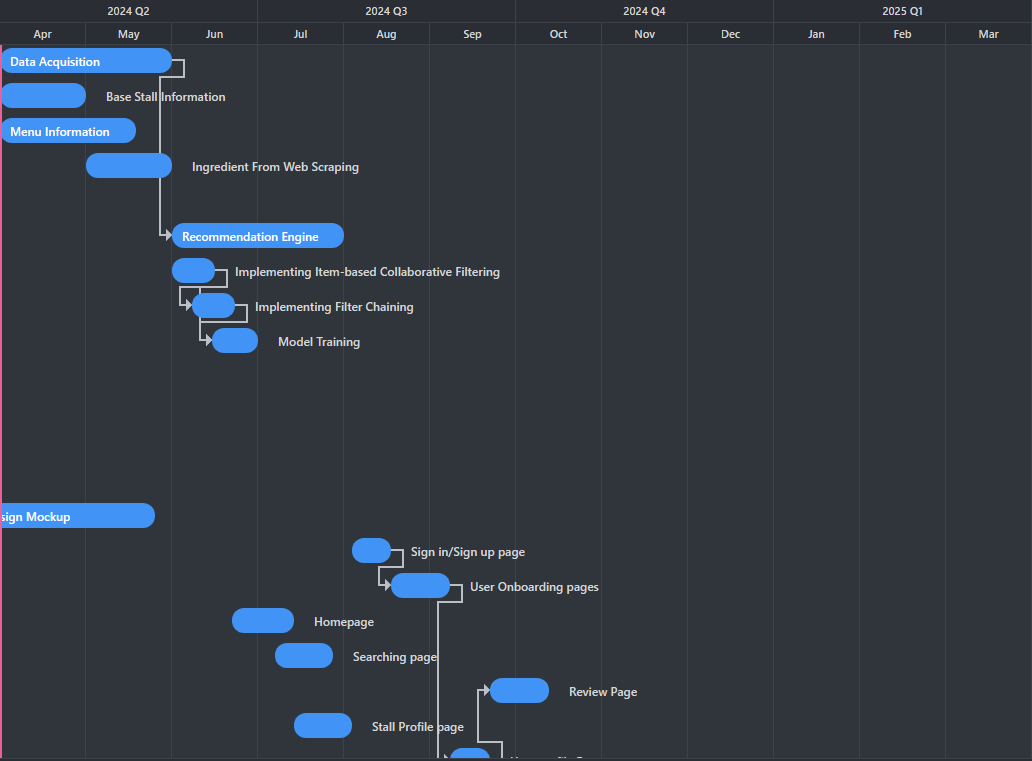
\includegraphics[width=\textwidth,height=0.5\textheight,keepaspectratio]{kueater/gantt-kueater.png}
    \caption{Timeline for KU Eater Project}
    \label{fig:timeline}
\end{figure}

As shown in figure \ref{fig:timeline}, it represents the timeline\footnote{Timeline is available online at: \url{https://sharing.clickup.com/9018244831/g/h/8crezpz-58/07a558d567cc98e}} of project.
KU Eater started with user interface design at the end of March 2024, and our data acquisition process is on April-May 2024. Starting from June 2024, we develop
the recommendation engine and other artificial intelligence components; along with implementing the application based on the design.

Our first deployment is on December 2024, and continously take feedback from users for later improvement during January-February 2025. The final project
will be published on March 2025.

\section{Terminology}
\label{section:terminology}

\begin{itemize}[leftmargin=40pt]
    \item \textbf{\textit{Artificial Intelligence (AI)}}---a technology that enables computers and machines to imitate complex human skills.
    \item \textbf{\textit{Machine Learning (ML)}}---a process involving training computers with sets of data to develop an ability to learn without explicit instructions. It involves uses of complex mathematical algorithms and statistical models to draw inferences from patterns in data.
    \item \textbf{\textit{Personalization}}---a feature or an ability of software to allow users to customize their experience with variables or context given by the users.
    \item \textbf{\textit{Sentiment Analysis}}---a process of analyzing digital text to determine if the emotional tone of the message is positive, negative, or neutral.
\end{itemize}